\documentclass[10pt,twocolumn]{article}

\usepackage{times}
\usepackage{fullpage}

\usepackage{graphicx}
\usepackage{amssymb}
\usepackage{algorithm}
\usepackage[noend]{distribalgo}
\usepackage{fixme}
\usepackage{alltt}
\usepackage{xspace}
\usepackage{adjustbox}
\usepackage[usenames,dvipsnames,svgnames,table]{xcolor}
\usepackage[dvipsnames]{xcolor}
\usepackage{caption}
\usepackage{subcaption}

\newcommand{\ex}{$\mathcal{E}$}
\newcommand{\pp}{$\mathcal{P}$}
\newcommand{\ppm}{\mathcal{P}}
\newcommand{\pqm}{\mathcal{Q}}
\newcommand{\oom}{\mathcal{O}}
\newcommand{\oo}{$\mathcal{O}$}
\newcommand{\cc}{$\mathcal{C}$}
\newcommand{\ccm}{\mathcal{C}}
\newcommand{\kk}{$\mathcal{K}$}
\newcommand{\vv}{$\mathcal{V}$}
\newcommand{\vvm}{\mathcal{V}}
\newcommand{\vvt}{$\mathcal{V}$}
\newcommand{\rr}{$\mathcal{R}$}
\newcommand{\rrm}{\mathcal{R}}
\newcommand{\sst}{$\mathcal{S}$}
\newcommand{\ssm}{\mathcal{S}}
\newcommand{\ip}{\mathcal{I}}
%
% S-SMR
\newcommand{\ssmr}{\mbox{S-SMR}\xspace}
\newcommand{\ssmrshort}{Scalable SMR}
\newcommand{\ssmrlong}{Scalable State Machine Replication}
%
% DS-SMR
\newcommand{\dssmr}{\mbox{DS-SMR}}
\newcommand{\dssmrshort}{Dynamic S-SMR}
\newcommand{\dssmrlong}{Dynamic Scalable State Machine Replication}
%
% The new DS-SMR system
\newcommand{\dynastar}{\mbox{DynaStar}\xspace}

\newcommand{\libname}{DynaStar} 
\newcommand{\appname}{Chirper}
%
\newcommand{\rmcast}{r-mcast}
\newcommand{\rmdel}{r-deliver}
\newcommand{\amcast}{a-mcast}
\newcommand{\amdel}{a-deliver}
\newcommand{\parts}{partition}
\newcommand{\coloralgo}{Yellow}

\newcommand{\mynote}[3]{
   \fbox{\bfseries\sffamily\scriptsize#1}
   {\small$\blacktriangleright$\textsf{\emph{\color{#3}{#2}}}$\blacktriangleleft$}}
\newcommand{\fp}[1]{\mynote{Fernando}{#1}{Red}}
\newcommand{\eb}[1]{\mynote{Eduardo}{#1}{Green}}
\newcommand{\ef}[1]{\mynote{Enrique}{#1}{Blue}}
\newcommand{\lle}[1]{\mynote{Long}{#1}{Cerulean}}
\newcommand{\rjs}[1]{\mynote{Robert}{#1}{Gold}}

\newcommand{\red}[1]{\textit{\textcolor{red}{#1}}}

% % do not change these values
% \baselineskip 12pt
% \textheight 9in
% \textwidth 6.5in
% \oddsidemargin 0in
% \topmargin 0in
% \headheight 0in
% \headsep 0in

\begin{document}

\title{\dynastar: Optimized Dynamic Partitioning for\\ Scalable State Machine Replication}
\author{Long Hoang Le$^1$, Enrique Fynn$^1$, Mojtaba Eslahi-Kelorazi$^1$, Robert Soul\'{e}$^1$ and Fernando Pedone$^1$ \\
\small {\em  $^1$University of Lugano} \\ [2mm]
\small Submission Type: Research
}
\date{}
\maketitle

\thispagestyle{empty}

\begin{abstract}
  
Classic state machine replication (SMR) does not scale well, since
each replica must execute every command.  To address this problem,
several systems have investigated the use of state partitioning in the
context of SMR, allowing client commands to be executed on a subset of
replicas. Prior approaches range from completely static schemes, which do not
adapt as workloads change, to dynamic schemes, which move data on-demand.


This paper presents DynaStar, a new dynamic partitioning scheme for
scaling state machine replication. In contrast to prior dynamic
schemes, DynaStar uses a replicated location oracle to maintain a global view
of the workload and inform heuristics about data placement. Using this
oracle, DynaStar can adapt to workload changes over time,
while also minimizing the number of state moves. The result is a
practical technique that achieves excellent performance.



\end{abstract}

%!TEX root =  main.tex
\section{Introduction}


\begin{figure*}[ht!]
  \centering
  \begin{subfigure}[b]{0.45\textwidth}
    \centering
    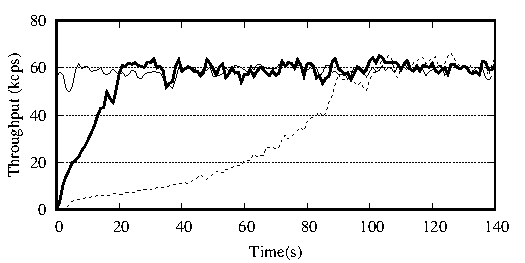
\includegraphics[width=0.95\columnwidth]{figures/experiments/dynastar-vs-dssmr-4p-0-tp}
    \caption{Throughput with strong locality}
  \end{subfigure}
  \begin{subfigure}[b]{0.45\textwidth}
    \centering
    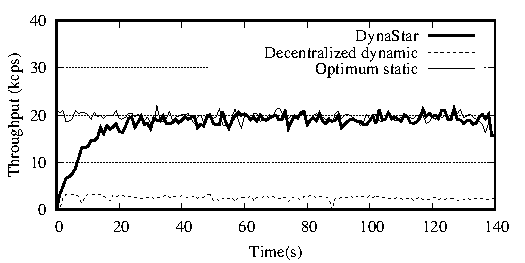
\includegraphics[width=0.95\columnwidth]{figures/experiments/dynastar-vs-dssmr-4p-5-tp}
    \caption{Throughput with weak locality}
  \end{subfigure} \\
  \begin{subfigure}[b]{0.45\textwidth}
    \centering
    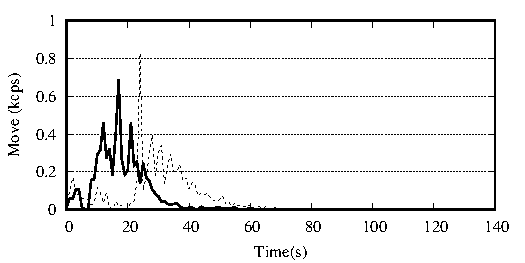
\includegraphics[width=0.95\columnwidth]{figures/experiments/dynastar-vs-dssmr-4p-0-move}
  \caption{Number of move commands with strong locality}
  \end{subfigure}
  \begin{subfigure}[b]{0.45\textwidth}
    \centering
    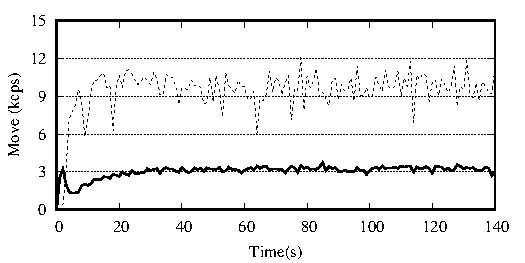
\includegraphics[width=0.95\columnwidth]{figures/experiments/dynastar-vs-dssmr-4p-5-move}
    \caption{Number of move commands with weak locality}
  \end{subfigure}
  \caption{\dynastar, optimum static and decentralized dynamic schemes under strong and weak locality (4 partitions).}
  \label{fig:motivation}
\end{figure*}




State machine replication (SMR) is a fundamental technique for
building fault-tolerant systems and services. With SMR, state is
replicated on a set of servers and each replica deterministically
executes the same sequence of client commands in order to maintain
consistency~\cite{Lam78,Sch90}. Unfortunately, classic state machine replication does not
scale, since each replica must execute every command. In order to
improve the scalability of SMR, several systems have investigated the
use of state partitioning~(e.g., \cite{corbett2013spanner, bezerra2014ssmr,Glendenning:2011kj,
  Aguilera:2007,bli16edcc}).

In principle, increasing the number of partitions should result in
increased system performance. However, if the execution of commands involves
multiple partitions, then performance can
actually decrease, due to overhead from ordering and coordinating
commands across partitions to ensure strong consistency. Moreover, if
data is not distributed carefully, then load imbalances can nullify
the benefits of partitioning. Thus, an ideal partitioning scheme is
one that would both (i) allow commands to be executed at a single
partition only, and (ii) evenly distribute data so that load is
balanced among partitions.  We refer to workloads that can be
partitioned in a way that satisfies these two properties as exhibiting
\emph{strong locality}.
Conversely, workloads that cannot avoid multi-partition commands with balanced load among partitions exhibit \emph{weak locality}.

Broadly speaking, there are two classes of techniques for
partitioning: \emph{static} and \emph{dynamic}.
Figure~\ref{fig:motivation} shows the result of a motivating
experiment that compares two representative systems, one of each class. In the
experiment, we measured the throughput and number of state moves over
time with two different workloads: one with strong locality and one
with weak locality. The workloads are inspired by the social network
Twitter, in which the network is modeled as a graph, and users can
``post'' messages. The social graph was generated using a Zipfian
distribution, where the Zipf parameter was adjusted to alter the
locality.  For brevity, we postpone the details of the experimental
setup until Section~\ref{sec:experiments}.


Static techniques choose an immutable assignment of application state variables to partitions
prior to executing commands. As an example of a static approach for
use in the experiment, we modified the S-SMR
system~\cite{bezerra2014ssmr} to use the static
METIS~\cite{Abou-Rjeili:2006} partitioning algorithm.  The METIS
algorithm is optimized to minimize edge-cuts when partitioning a
static social graph. 
In the workload with strong locality, METIS partitions the social graph such that all posts are single partition;
in the workload with weak locality, although most commands are single partition, a small fraction of posts involves multiple partitions.
As expected, we see that the throughput is less
for the weak locality workload, due to the more expensive execution of multi-partition posts.
%since the static scheme incurs overhead when accessing multiple partitions to execute commands.
For workloads that do not change the graph structure, the
results in Figure~\ref{fig:motivation} show a theoretical maximum
throughput.  Of course, these results are not achievable in practice,
since for real workloads, the graph would change over time (e.g., in
social networks users join and leave the system, connections are
created and removed).


Dynamic techniques address the limitations of static techniques by adapting
the partitioning scheme as workloads change.  
For example, a dynamic technique can move data ``on demand'' to maximize the number of single partition user commands, while avoiding imbalances in the load of the partitions.  
%Typically, this is
%implemented by moving data ``on demand'' to a single partition which
%executes a user command.  
The major challenge in designing a dynamic
scheme is determining how the system selects the partition to which to
move data.
%
The second system in Figure~\ref{fig:motivation} evaluates the dynamic
partitioning strategy implemented by  Long et al.~\cite{hoang2016}.
This system selects partitions randomly, which allows for a completely 
decentralized implementation, in which partitions make only local
choices about data movement.  We refer to this approach as
\emph{decentralized dynamic}.  As Figure~\ref{fig:motivation} shows,
the {decentralized dynamic approach works well for data with strong
  locality, but is unstable for workloads with weak locality, since
  data is constantly moved from one partition to another.


In this paper, we introduce \dynastar, a new dynamic approach to the
state partitioning problem.  Like other dynamic approaches, \dynastar
does not require any a priori knowledge about the workload. However,
\dynastar differs from prior approaches because it maintains a
location oracle with a global view of the network.  The oracle minimizes the
number of state relocations by monitoring the workload, and
re-computing an optimized partitioning on demand using a static
partitioning algorithm.  As a preview of our results,
Figure~\ref{fig:motivation} also includes measurements for \dynastar.
We see that \dynastar is able to achieve throughputs comparable to
the optimized static scheme, while adapting to workload changes
on-the-fly, and preserving strong consistency.


With \dynastar, a location oracle maintains two data structures: (i) a
mapping of application state variables to partitions, and (ii) a \emph{workload graph}
with state variables as vertices and edges as commands that access the
variables.  When a client submits a command, it must first contact the
location oracle to discover the partitions on which state variables are
stored.  If the command accesses variables in multiple partitions, the
oracle issues a move command to the partitions, re-locating variables to
a single partition. Of course, when re-locating a variable, the oracle
is faced with a choice of which partition to use as a destination.
\dynastar chooses the partition for relocation (i.e., one that
would minimize the number of state relocations) by partitioning the
workload graph using the METIS partitioner.
%Although METIS does not necessarily produce the best possible partitioning of the workload graph, it offers a good compromise between performance and partitioning quality.

To tolerate failures, \dynastar implements the oracle as a regular partition, replicated in a set of nodes.
To ensure that the oracle does not become a performance bottleneck, clients cache location information.
Therefore, clients only query the oracle when they access a variable for the first time or when cached entries become invalid (i.e., because a variable changed location).
\dynastar copes with commands addressed to wrong partitions by telling clients to retry a command.

%\rjs{Should we say something about the location oracle not being a bottleneck?}

We have fully implemented \dynastar and compared its performance to
the dynamic partitioning protocol proposed by Long et
al.~\cite{hoang2016} and to the optimized static partitioning scheme.
%Our prototype can handle workload graphs with half a million variables
%and tens of millions of connections. \ef{Not yet :-|}
In workloads that present strong
locality, all three protocols eventually delivered comparable
performance, although \dynastar converged more quickly than the
decentralized scheme.  In workloads with weak locality,
\dynastar largely outperformed the decentralized scheme and performed
similar to the optimized static partitioning scheme.

%The reason for the surprisingly high performance of \dynastar compared to the optimized
%static partitioning scheme is that 
%\textbf{we need to explain this!!!
%:-)} \ef{If the cost of migrating the object outperforms the cost of 
%signaling partitions, why performance get similar when we have more partitions?} 
%\lle{in static scheme, partitions exchange signal in every global commands,
%while, in dynamic scheme, there is chance that partitions already have
%data, thus no communication needed. More over, signaling is a two-way mechanism,
%while moving objects in dynamic scheme is only one-way, which leads to less data
%is being exchanged}

The paper makes the following contributions:
\begin{itemize}
\item It introduces \dynastar and discusses its implementation. 
\item It evaluates different partitioning schemes for state machine replication under a variety of conditions.
\item It describes \appname{} to demonstrate how \dynastar can be used to implement a scalable social network service.
\item It presents a detailed experimental evaluation of \dynastar
%including real social network graphs with half a million users and 14 million edges.
\end{itemize}

The rest of the paper is structured as follows.
Section~\ref{sec:sysmodel} presents the system model.
Section~\ref{sec:background} reviews existing scalable state machine replication approaches.
Section~\ref{sec:dynastar} introduces \dynastar, describes the technique in detail and argues about its correctness.
Section~\ref{sec:implementation} overviews our prototype.
Section~\ref{sec:experiments} reports on the results of our experiments.
Section~\ref{sec:rw} surveys related work and
Section~\ref{sec:conclusion} concludes the paper.




%% %% Because single-partition commands are much more efficient than
%% %% multi-partition commands (i.e., in some cases by a factor of more than
%% %% 10x), the performance of a distributed storage system is particularly sensitive to the way
%% %% the service state is partitioned.


%% \subsection{State Machine Replication}

%% State machine replication (SMR) is a well-established technique to
%% develop highly available services (e.g.,
%% \cite{Shvachko:2003,Ghemawat:2003,Burrows:2006,MacCormick:2004}).  In
%% essence, the idea is that replicas deterministically execute the same
%% sequence of client commands in the same order and in doing so traverse
%% the same sequence of states and produce the same results.  State
%% machine replication provides configurable fault tolerance in the sense
%% that the system can be set to tolerate any number of faulty replicas.
%% Increasing the number of replicas, however, will not scale performance
%% since each replica must execute every command.  Unfortunately,
%% increasing the number of replicas will not scale performance since
%% each replica must execute every command.

%% S-SMR relies on an atomic multicast primitive to consistently order
%% commands within and across partitions.  Commands that access objects
%% located in a single partition (i.e., single-partition commands) are
%% multicast to the concerned partition and executed like in classical
%% SMR.  Commands that access objects located in multiple partitions
%% (i.e., multi-partition commands) are multicast to all involved
%% partitions.  To prevent command interleaves that violate strong
%% consistency, partitions coordinate during the execution of
%% multi-partition commands.



%% \subsection{Motivating Example}

%!TEX root =  main.tex
\section{System model and definitions}
\label{sec:sysmodel}

\dynastar relies on multicast abstractions to handle complex coordination among partitions without violating correctness. 
In this section, we detail the system model, define multicast, and state our correctness criterion. 

\subsection{Processes and communication}

We consider a distributed system consisting of an unbounded set of
client processes $\ccm = \{c_1, c_2, ...\}$ and a bounded set of
server processes (replicas) $\ssm = \{s_1, ..., s_n\}$.  Set $\ssm$ is
divided into disjoint groups of servers $\ssm_0, ..., \ssm_k$.
Processes are either \emph{correct}, if they never fail, or
\emph{faulty}, otherwise.  In either case, processes do not experience
arbitrary behavior (i.e., no Byzantine failures).

Processes communicate by message passing, using either one-to-one or
one-to-many communication.  The system is asynchronous: there is no
bound on message delay or on relative process speed.  One-to-one
communication uses primitives $send(p,m)$ and $receive(m)$, where $m$
is a message and $p$ is the process $m$ is addressed to.  If sender
and receiver are correct, then every message sent is eventually
received.
%
One-to-many communication relies on reliable multicast and atomic
multicast,\footnote{Solving atomic multicast requires additional
  assumptions~\cite{CT96,FLP85}. In the following, we simply assume
  the existence of an atomic multicast oracle.} defined in
\S\ref{sec:rmcast} and \S\ref{sec:amcast}, respectively.


\subsection{Reliable multicast}
\label{sec:rmcast}

To reliably multicast a message $m$ to a set of groups $\gamma$,
processes use primitive \rmcast$(\gamma, m)$.  Message $m$ is
delivered at the destinations with \rmdel$(m)$.  Reliable multicast
has the following properties:

\begin{itemize}

    \item[--] If a correct process \rmcast{}s $m$, then every correct
      process in $\gamma$ \rmdel{}s $m$ \emph{(validity)}.
    
    \item[--] If a correct process \rmdel{}s $m$, then every correct
      process in $\gamma$ \rmdel{}s $m$ \emph{(agreement)}.
    
    \item[--] For any message $m$, every process $p$ in $\gamma$
      \rmdel{}s $m$ at most once, and only if some process has
      \rmcast{} $m$ to $\gamma$ previously \emph{(integrity)}.
    
\end{itemize}

\subsection{Atomic multicast}
\label{sec:amcast}

To atomically multicast a message $m$ to a set of groups $\gamma$,
processes use primitive \amcast$(\gamma, m)$.  Message $m$ is
delivered at the destinations with \amdel$(m)$.  We define delivery
order $<$ as follows: $m < m'$ iff there exists a process that
delivers $m$ before $m'$.

Atomic multicast ensures the following properties:

\begin{itemize}
    
    \item[--] If a correct process \amcast{}s $m$, every correct
      process in a group in $\gamma$ \amdel{}s $m$ \emph{(validity)}.
    
    \item[--] If a process \amdel{}s $m$, then every correct process
      in a group in $\gamma$ \amdel{}s $m$ \emph{(uniform agreement)}.
    
    \item[--] For any message $m$, every process \amdel{}s $m$ at most
      once, and only if some process has \amcast{} $m$ previously
      \emph{(integrity)}.
    
    \item[--] If a process \amcast{}s $m$ and then $m'$, then no process \amdel{}s $m'$ before $m$ \emph{(fifo order)}.

    \item[--] The delivery order is acyclic \emph{(atomic order)}.

    \item[--] For any messages $m$ and $m'$ and any processes $p$ and
      $q$ such that $p \in g$, $q \in h$ and $\{ g, h \} \subseteq
      \gamma$, if $p$ delivers $m$ and $q$ delivers $m'$, then either
      $p$ delivers $m'$ before $m$ or $q$ delivers $m$ before $m'$
      \emph{(prefix order)}.
    
\end{itemize}

Atomic broadcast is a special case of atomic multicast in which there
is a single group of processes.

\subsection{Correctness criterion}
\label{sec:correctcrit}

Our consistency criterion is linearizability.  A system is
\emph{linearizable} if client commands can be reordered
in a sequence that (i)~respects the semantics of the commands, as
defined in their sequential specifications, and (ii)~respects the
real-time precedence of commands~\cite{Attiya04}.



%!TEX root =  main.tex
\section{Background}
\label{sec:background}


\dynastar builds on prior work on classic state machine replication and scalable state machine replication.
% (e.g.,~\cite{bezerra2014ssmr,hoang2016}) 
In this section, we briefly review these techniques. 

\subsection{State machine replication}
\label{sec:smr}

State machine replication is a fundamental approach to fault tolerance.
It replicates servers and coordinates the execution of client commands at replicas~\cite{Lam78,Sch90}. 
Every replica has a full copy of the service state, identified by a set of state variables $\vvm = \{v_1, ..., v_m\}$.
A command is a sequence of deterministic operations that can read and modify the state.
By starting in the same initial state and executing the same sequence of deterministic commands in the same order, servers make the same state changes and produce the same reply for each command. 
To guarantee that servers deliver the same sequence of commands, SMR can be implemented with atomic broadcast: commands are atomically broadcast to all servers, and all correct servers deliver and execute the same sequence of commands \cite{BJ87b,DSU04}.


\subsection{Scaling State Machine Replication}

Despite its simple execution model, classic SMR does not scale; adding resources (e.g., replicas) will not translate into sustainable improvements in throughput. 
Several approaches have been proposed to address SMR's scalability limitations.
In all proposed protocols, the idea is to shard the service's state and replicate each shard.
More precisely, the service state \vvt\ is composed of $k$ partitions, $\ppm_1, ..., \ppm_k$, where each partition $\ppm_i$ is assigned to server group $\ssm_i$. 
(For brevity, we say that server $s$ belongs to $\ppm_i$ meaning that $s \in \ssm_i$.)
%, and say ``multicast to $\ppm_i$" meaning ``multicast to server group $\ssm_i$".
%
Commands that access a single partition are executed as in classic SMR.
%: replicas of the concerned partition agree on the execution order and each replica executes the command independently. 
Existing protocols differ in (a) how to handle multi-partition commands and (b) whether state partitioning is static or dynamic.

There are three approaches to handling multi-partition commands.
Some protocols assume a workload that can be ``perfectly partitioned," that is, there is a way to shard the service state that avoids multi-partition commands \cite{hoang2016,Nogueira17}.
Since commands are essentially single-partition, if the load is balanced across partitions then performance scales with the number of partitions.
With protocols that support commands that span multiple partitions, the multi-partition command is first ordered across the involved partitions (e.g., using an atomic multicast) and then executed by each involved partition.
Some protocols assume the workload can be sharded such that multi-partition commands are executed locally by each of the involved partitions \cite{Mu2016}, that is, the execution of a multi-partition command in one partition does not need data stored in a different partition.
For example, to support the assignment command ``$x := y$", variables $x$ and $y$ must be placed in the same partition.
However, a command that increments $x$ and increments $y$ allows these variables to be placed in different partitions.

More general solutions do not impose restrictions on state partitioning, but incur additional overhead in the execution of multi-partition commands \cite{bezerra2014ssmr, hoang2016}.
Upon delivering a multi-partition command, replicas may need to exchange state, since some partitions may not have all the variables needed in the command.
For example, consider again the assignment command ``$x := y$" in a system where $x$ and $y$ are stored in different partitions.
With S-SMR \cite{bezerra2014ssmr}, the partitions first exchange $x$ and $y$ and then both execute the command.
DS-SMR \cite{hoang2016} supports dynamic partitioning of state; thus, either $x$ is moved to the partition that contains $y$ or vice-versa, and the command is executed at a single partition.

None of the existing approaches discuss how to partition the state of a general service in order to minimize multi-partition commands and keep the load across partitions balanced.
DS-SMR \cite{hoang2016} achieves these goals for services that can be perfectly partitioned.
In the next section, we introduce \dynastar, a protocol that minimizes multi-partition commands and balances partition load without these restrictions. 


%!TEX root =  main.tex
\section{\dynastar}
\label{sec:dynastar}

%%In this section, we overview \dynastar's key ideas, present the protocol in detail, discuss some performance optimizations, and argue about \dynastar's correctness.
%\subsection{Key insights}
%
%\dynastar optimizes state partitioning based on the workload and relocates application state on-the-fly, without service disruption.
%\begin{itemize}
%\item \emph{Optimized state partitioning.}
%\dynastar models a service workload as a graph $G = (V, E)$, where vertices represent state variables and edges dependencies between variables.
%An edge connects two variables in the graph if a command accesses both of them.
%A location oracle builds the workload graph based on feedback from the clients or partitions, as commands are executed.
%The oracle periodically computes a partitioning of the workload graph and propagates the partitioning to the various partitions.
%
%\item \emph{On-the-fly relocation of service state.}
%Based on the partitioning computed by the oracle, servers determine the best partition to execute a multi-partition command.
%State is then temporarily moved on demand to the destination partition where the command will be executed.
%After the command is executed, updated variables are moved back to their source partition to keep the optimized partitioning.
%When the oracle computes a new partitioning of the data, state is relocated (i.e., variables moved from one partition to another) to reflect the new optimized partitioning. 
%\end{itemize}

%In \dynastar a move request is multicast together with the command that triggered the request.
%%a partition executes a command right after it has gathered all variables it needs.
%Therefore, differently from DS-SMR, \dynastar ensures termination without resorting to expensive mechanisms (i.e., S-SMR).

\subsection{Overview}

\dynastar defines a dynamic mapping of application variables to partitions.\footnote{Applications may also define other granularity of data when mapping application state to partitions. For example, in our social network application (\S\ref{sec:imp:\appname}), each user (together with the information associated with the user) is mapped to a partition; in our TPC-C implementation (\S\ref{sec:imp:tpcc}), every district in a warehouse is mapped to a partition.}
Such a mapping is managed by a partitioning oracle, which is handled as a replicated partition.
%The oracle allows the mapping of variables to partitions to be retrieved or changed during execution.
To simplify the discussion, we initially assume that every command involves the oracle.
In \S\ref{sec:optm}, we explain how clients can use a cache to avoid the oracle in the execution of most commands.

% REMOVE THIS?
%State is then temporarily moved on demand to the destination partition where the command will be executed.
%After the command is executed, updated variables are moved back to their source partition to keep the optimized partitioning.

Clients submit commands to the oracle and wait for the reply. 
\dynastar\ supports three types of commands:
$create(v)$ creates a new variable $v$ and initially maps it to a partition defined by the oracle;
$access(\omega)$ is an application command that reads and modifies variables in set $\omega \subseteq \vvm$; and
$delete(v)$ removes $v$ from the service state.
The reply from the oracle is called a $prophecy$, and usually 
consists of a set of tuples $\langle v, \ppm \rangle$, meaning 
$v \in \ppm$, and a target partition $\ppm_d$ on which the command 
will be executed. The $prophecy$ could also tell the clients 
if a command cannot be executed (e.g., it accesses 
variables that do not exist). If the command can be executed, 
the client waits for the reply from the target partition.

If a command $C$ accesses variables in $\omega$ on a single partition, 
the oracle multicasts $C$ to that partition for execution. If the command 
accesses variables on multiple partitions, the oracle multicasts a 
$global(\omega,\ppm_d, C)$ command to the involved partitions to gather 
all variables in $\omega$ to the target partition $\ppm_d$. After having all 
required variables, the target partition executes command $C$, 
sends the reply to the client, and returns the variables to their source. 

The oracle also collects hints from clients and partitions to 
build up a workload graph and monitors the changes in the graph. 
%\dynastar models a service workload as a graph $G = (V, E)$, where 
In the workload graph, vertices represent state variables and edges dependencies between variables.
An edge connects two variables in the graph if a command accesses both of them.
%A location oracle builds the workload graph based on feedback from the clients or partitions, as commands are executed.
Periodically, the oracle computes a new optimized partitioning and sends the partitioning plan to all partitions. 
Upon delivering the new partitioning, 
the partitions exchange variables and update their state accordingly.
\dynastar relocates variables without blocking the execution of commands.


\subsection{The detailed protocol}
\label{sec:detailed}

Algorithms~\ref{alg:client_proxy}, \ref{alg:oracle_proxy}, and \ref{alg:server_proxy} describe the client, oracle, and server processes, respectively. 
For brevity, we omit the delete command since the coordination involved in the create and delete commands are analogous. 


\subsubsection{The client process} 

To execute a command, the client atomically multicasts the command to the oracle (Algorithm 1).
The oracle replies with a prophecy, which may already tell the client that the command cannot be executed (e.g., it needs a variable that does not exist, it tries to create a variable that already exists).
If the command can be executed, the client receives a prophecy containing the partition where the command will be executed. The client then waits for the result of the execution of the command.


% The client must retry the command if the partition cannot execute the command.
% This happens if the cache on client is invalid, some of the variables needed by the command were moved to another partition due a new partitioning. 
%To ensure that a command is eventually executed, after retrying a few times, the client falls back to using \ssmr{}, multicasting the command to all partitions (and the oracle, in case of a create or delete command).


\subsubsection{The oracle} 

When the oracle delivers a request, it distinguishes between two cases (Task 1 in Algorithm~\ref{alg:oracle_proxy}).
\begin{itemize}
\item If the command is to create a variable $v$, and $v$ does not already exist, the oracle chooses a random partition for $v$, multicasts the create command to the partition and itself, and returns the partition to the client as a prophecy (Figure~\ref{fig:oracle_repartition}).
\item If the command reads and writes existing variables, the oracle first checks that all such variables exist.
If the variables exist and they are all in a single partition, the oracle multicasts the command to that partition for execution.
If the variables are distributed in multiple partitions, the oracle deterministically determines the destination partition, and atomically multicasts a command to the involved partitions so that all variables are gathered at the destination partition.
The oracle chooses as the destination partition the partition that contains most of the variables needed by the command.
(In case of a tie, one partition is chosen deterministically, among those that contain most variables.)
Once the destination partition has received all variables needed by the command, it executes the command and returns the variables to their source partition.

%In either case, oracle returns a prophecy back to the client with the destination partition.
\end{itemize}


\begin{algorithm}[h!]
\small

\begin{distribalgo}[1]

%\vspace{1.0mm}

\INDENT{\colorbox{\coloralgo}{To issue a command $C$, the client does:}}

\vspace{1.0mm}
	% \STATE $\omega \leftarrow vars(C)$
	% \COMMENT{variables accessed by $C$}

	% \IF[if $v$ $\neg$exists in cache:]{$\exists v \in \omega : cache(\{v\}) = \bot$}
		\STATE \amcast$($oracle, $exec(C))$
		% \COMMENT{multicast command to $oracle$}
		\STATE wait for $prophecy$
		\IF[if receive $nok$ then...]{$prophecy = nok$}
			\STATE $reply \leftarrow prophecy$
			\COMMENT{...there's nothing to execute}
		\ELSE[in this case, $prophecy$ is $(dest)$]
			% \STATE $cache(\{v\}) \leftarrow prophecy$
			\STATE wait for $reponse$ from a server in $prophecy$
			\STATE $reply \leftarrow reponse$
		\ENDIF
	% \ELSE[if all vars in $\omega$ exist in cache]
	% 	\STATE $\ppm_d \leftarrow target(G_W, \omega)$
	% 	\COMMENT{select partition to execute}
	% 	\STATE \amcast$(\ppm_d, exec(C))$
	% 	\STATE wait for $reponse$ from server $\ppm_d$
	% 	\IF[if receive $retry$ then...]{$reponse = retry$}
	% 		\STATE $cache(\{v\}) \leftarrow \bot$
	% 		\COMMENT {clear cache of $\omega$}
	% 		\STATE return retry $C$
	% 	\ELSE
	% 		\STATE $reply \leftarrow reponse$
	% 	\ENDIF	

	% \ENDIF
\STATE return $reply$ to the application

\vspace{1.0mm}

% \INDENT{\colorbox{\coloralgo}{\textbf{function} cache$(vars)$}}
% 	\STATE $dests \leftarrow \{ \ppm : \exists v \in vars \cap \ppm \}$
% 	\STATE return $dests$
% \ENDINDENT

% \vspace{1.0mm}
% \INDENT{\colorbox{\coloralgo}{\textbf{function} target$(vars)$}}
% 	\STATE $\ppm \leftarrow$ compute destination partition for $vars$ from\\ \hspace{8mm}current $\ppm_1, ..., \ppm_m$ and $\ip_1, ..., \ip_m$ partitioning
% 	\STATE return $\ppm$
% \ENDINDENT	

\ENDINDENT

\caption{Client}
\label{alg:client_proxy}
\end{distribalgo}
\end{algorithm}
\begin{algorithm}[t!]
\small

\begin{distribalgo}[1]

%\vspace{1.0mm}

\INDENT[\textbf{Task 1}]{\colorbox{\coloralgo}{\textbf{when} \amdel$(exec(C))$}}
	\INDENT{\textbf{case} $C$ is a $create(v)$ command:}
		\IF[if $v$ already exists...]{$\parts(\{v\}) \neq \bot$}
			\STATE $prophecy \leftarrow nok$
			\COMMENT{...notify client}
		\ELSE[if $v$ doesn't exist...]
			\STATE $\ppm \leftarrow$ choose $v$'s partition
			\COMMENT{...determine $v$'s partition}
			\STATE $prophecy \leftarrow \ppm$
			\COMMENT{prepare client's response}
			\STATE $alldest \leftarrow \{oracle\} \cup \{ \ppm \}$
			\STATE \amcast$(alldest, (\ppm,create(v)))$
%					\COMMENT{send command to partition}
		\ENDIF
	\ENDINDENT

	\INDENT{\textbf{case} $C$ is any command, but $create(v)$:}
		\STATE $\omega \leftarrow vars(C)$
		\COMMENT{variables accessed by $C$}
		\IF[if $v$ $\neg$exists:]{$\exists v \in \omega : \parts(\{v\}) = \bot$}
			\STATE $prophecy \leftarrow nok$
			\COMMENT{tell the client}
		\ELSE[if all vars in $\omega$ exist]
			\STATE $dests \leftarrow \parts(\omega)$
			\COMMENT{get all partition involved}
			\STATE $\ppm_d \leftarrow target(dests, C)$
			\COMMENT{$\ppm_d$ will excecute $C$}
			\STATE \amcast$(dests, C)$
			\STATE $prophecy \leftarrow \ppm_d$
		\ENDIF
	\ENDINDENT
	\STATE send $prophecy$ to the client
\ENDINDENT
\vspace{1.0mm}

\INDENT[\textbf{Task 2}]{\colorbox{\coloralgo}{\textbf{when} \amdel$(\ppm_v,create(v))$}}
%	\INDENT{\textbf{case} $C$ is a $create(v)$ command:}
%	\STATE \rmcast$(\ppm_v, \langle signal, C \rangle )$
	\STATE $\forall x \in \ppm_v$: send $(\langle signal, C \rangle )$ to $x$
	\COMMENT{exchange signal...}
	\STATE wait until $\langle signal, C \rangle \in rcvd\_msgs$
	\COMMENT{...to coordinate}
	\STATE $\ppm_v \leftarrow \ppm_v \cup      \{v\}$
% \STATE send $ok$ to the client
\ENDINDENT


\vspace{1.0mm}
\INDENT[\textbf{Task 3}]{\colorbox{\coloralgo}{\textbf{when} receive $( \langle val, C \rangle )$}}
%\INDENT[\textbf{Task 3}]{\colorbox{\coloralgo}{\textbf{when} \rmdel$( \langle val, C \rangle )$}}
	\STATE $rcvd\_msgs \leftarrow rcvd\_msgs \cup \{\langle val, C \rangle\}$
\ENDINDENT

\vspace{1.0mm}
\INDENT{\colorbox{\coloralgo}{\textbf{function} \parts$(vars)$}}
	\STATE $dests \leftarrow \{ \ppm : \exists v \in vars \cap \ppm \}$
	\STATE return $dests$
\ENDINDENT

	\vspace{1.0mm}

\INDENT[\textbf{Task 4}]{\colorbox{\coloralgo}{\textbf{when} \amdel$(hint(V_h,E_h))$}}
	\STATE update $G_W$ with $(V_h,E_h)$
	\STATE $inc(changes)$
	\IF {$changes \geq threshold$}
		\STATE $partitioning  \leftarrow$ compute $\ip_1, ..., \ip_m$ from $G_W$
		\STATE $alldest \leftarrow \{oracle\} \cup all partitions$
		\STATE \amcast$(alldest, (partitioning))$
	\ENDIF
\ENDINDENT

\vspace{1.0mm}

\INDENT[\textbf{Task 5}]{\colorbox{\coloralgo}{\textbf{when} \amdel$(\mathit{partitioning})$}}
	\STATE apply $partitioning$
\ENDINDENT

\vspace{1.0mm}

\INDENT{\colorbox{\coloralgo}{\textbf{function} target$(\ppm, C)$}}
	\STATE $\ppm_d \leftarrow$ deterministicly compute partition to execute\\ \hspace{8mm} command $C$ from $\forall \ppm_i \in \ppm$
	\STATE return $\ppm_d$
\ENDINDENT	

\vspace{1.5mm}

\textbf{Algorithm variables:}

\vspace{1mm}

$G_W$: the set of all variable and their locations

$partitioning$: the partition configuration of $G_W$


\caption{Oracle}
\label{alg:oracle_proxy}
\end{distribalgo}
\end{algorithm}




\begin{algorithm}[t!]
\small

\begin{distribalgo}[1]

\INDENT[\textbf{Task 1}]{\colorbox{\coloralgo}{\textbf{when} \amdel$(access(\omega))$}}
	% \IF{$\forall v \in \omega : v \in \ppm$}
		\STATE execute command $access(\omega)$
		\STATE send response to the client
	% \ELSE
		% \STATE send $retry$ to the client
	% \ENDIF
\ENDINDENT
\vspace{1.0mm}
	\INDENT[\textbf{Task 2}]{\colorbox{\coloralgo}{\textbf{when} \amdel$(move(\omega,dests,\ppm_d), access(\omega))$}}
%	\INDENT{\textbf{case} $C$ is a $move(v,\ppm_s,\ppm_d)$ command:}
		\IF[if $\ppm$ is a source partition:]{$\ppm \in dests \setminus \ppm_d$}
			\STATE $vars \leftarrow \omega \cap \ppm$
			\COMMENT{all needed variables in $\ppm$}
			\STATE \rmcast$(\ppm_d$,$\langle vars, C \rangle)$
			\COMMENT{send variables to destination}
			\STATE $\ppm \leftarrow \ppm \setminus \omega$
			\COMMENT{update source partition}
		\ELSE[$\ppm$ is destination partition:]
			\STATE wait until $\exists vars : \langle vars, C \rangle \in rcvd\_msgs$
				\STATE $\ppm \leftarrow \ppm \cup vars$
				\COMMENT{update partition}
				\STATE execute command $access(\omega)$
				\STATE send response to the client
		\ENDIF
	\ENDINDENT
	\vspace{1.0mm}
	\INDENT[\textbf{Task 3}]{\colorbox{\coloralgo}{\textbf{when} \amdel$(create(v))$}}
		\STATE $\ppm \leftarrow \ppm \cup \{v\}$
		\STATE send $ok$ to the client
	\ENDINDENT
%	\vspace{1.0mm}
%	\INDENT{\textbf{case} $C$ is a $delete(v)$ command:}
%		\STATE wait until $\langle val, C \rangle \in rcvd\_msgs$
%                \STATE $\ppm \leftarrow \ppm \setminus \{v\}$
%                \STATE send $ok$ to the client
%		\STATE \rmcast$(oracle, \langle ok, C \rangle )$
%        	\ENDINDENT
%\ENDINDENT

  \vspace{1.0mm}

  \INDENT[\textbf{Task 4}]{\colorbox{\coloralgo}{\textbf{when} \rmdel$( \langle val, C \rangle )$}}
      \STATE $rcvd\_msgs \leftarrow rcvd\_msgs \cup \{\langle val, C \rangle\}$
  \ENDINDENT

%\ENDINDENT

\caption{Server in partition $\ppm$}
\label{alg:server_proxy}
\end{distribalgo}
\end{algorithm}

\begin{figure*}
\begin{minipage}[b]{1\linewidth} % A minipage that covers the whole width of the page
\centering
      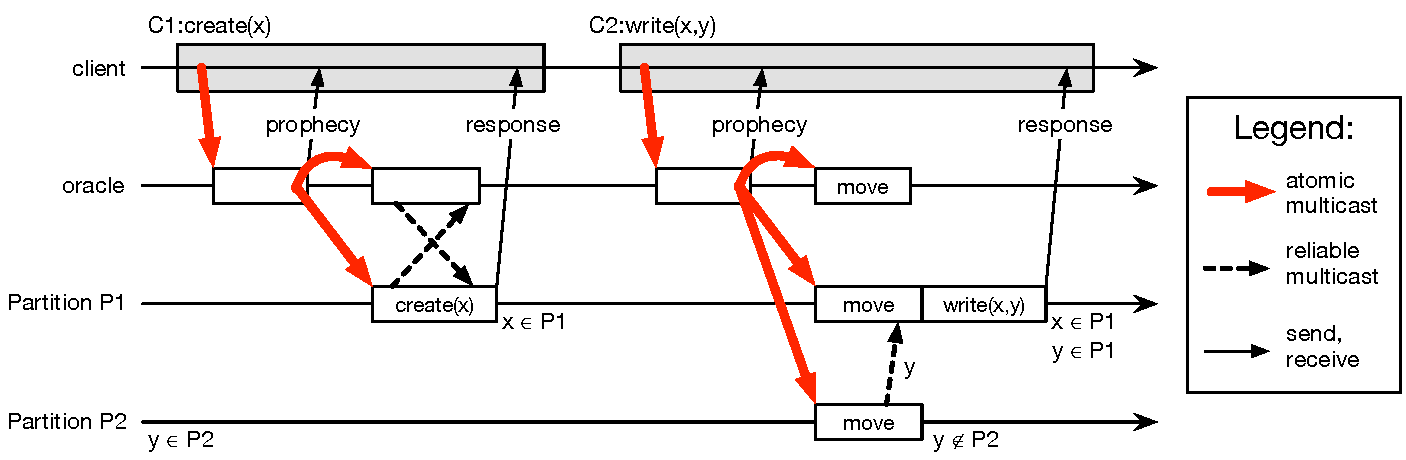
\includegraphics[width=\linewidth]{figures/dynastar}
\end{minipage}
\caption{The execution of a create (C1) and a write without client cache (C2) and with client cache (C3) in \dynastar.}
\label{fig:oracle_repartition}
\end{figure*}

Upon delivering a create (Task 2), the oracle updates its partition information.
As part of a create command, the oracle coordinates with the partition to ensure correctness (Task 3)~\cite{bezerra2014ssmr}.
%
The oracle also keeps track of the workload graph by receiving hints with variables (i.e., vertices in the graph) and executing commands (i.e., edges in the graph). These hints can be submitted by the clients or by the partitions, which collect data upon executing commands and periodically inform the oracle (Task 4).
The oracle computes a partitioning plan of the graph and multicasts it to all servers and to itself. Upon delivering new partition plan, the oracle updates its location map accordingly (Task 5).
% The oracle also keeps track of the workload graph, computes a partitioning of the graph, and determines the destination partition for move operations.
% To maintain the workload graph (Task 5), the oracle receives hints with variables (i.e., vertices in the graph) and executed commands (i.e., edges in the graph).

To compute an optimized partitioning, the oracle uses a graph partitioner.
A new partitioning can be requested by the application, by a partition, or by the oracle itself (e.g., upon delivering a certain number of hints).
To determine the destination partition of a set of variables, as part of a move, the oracle uses 
% the current location of variables and 
the last computed partitioning.

\subsubsection{The server process} 

When a server delivers a command $C$, it first checks if it has all variables needed by the command. If the server has all such variables, it executes the command and sends the response back to the client (Tasks 1a and 2 in Algorithm~\ref{alg:server_proxy}).
If not all the variables needed by the command are in that partition, the server runs a deterministic function to determine the destination partition to execute the command (Task 1b). The function uses as input the variables needed by the command and the command itself.
In this case, each server that is in the multicast group of the command $C$ but is not the destination partition sends all the needed variables stored locally to the destination partition and waits to receive them back. 
The destination partition waits for a message from other partitions. Once all variables needed are available, the destination partition executes the command $C$, sends the response back to the client, and returns the variables to their source.
Periodically, the servers deliver a new partitioning plan from the oracle (Task 3). Each server will send the variables to the designated partition, as in the plan, and wait for variables from other partitions. Once a server receives all variables, it updates its location map accordingly.
%When a server delivers a message to create a variable (and similarly to delete an existing variable), it coordinates with the oracle (Task 3).
%The exchange of signals between the partition where the variable will be created and the oracle ensures that interleaved executions between create and delete commands will not lead to violations of linearizability (i.e., this is essentially the execution of a multi-partition command involving the oracle and a partition~\cite{bezerra2014ssmr}).
To determine the destination partition for a command, the servers uses the last computed partitioning.


\subsection{Performance optimization}
%\subsection{Performance optimizations}
\label{sec:optm}

%We now describe two performance optimizations.
%
%\textbf{Caching.} 
In the algorithm presented in the previous section, clients always need to involve the oracle, and the oracle dispatches every command to the partitions for execution.
Obviously, if every command involves the oracle, the system is unlikely to scale, as the oracle will likely become a bottleneck.
To address this issue, clients are equipped with a location cache.
Before submitting a command to the oracle, the client checks its location cache.
If the cache contains the partition of the variables needed by the command, the client can atomically multicast the command to the involved partition and thereby avoid contacting the oracle. 

The client still needs to contact the oracle in one of these situations:
%(a)~according to client's cache, not all variables accessed by the command are in the same partition and it is necessary to move variables;
%(b)~the cache contains outdated information, and the command is multicast to a partition that does not contain all needed variables; or
(a)~the cache contains outdated information; or
(b)~the command is a create, in which case it must involve the oracle, as explained before.
%If the cache contains outdated information and the addressed partition does not contain all the variables accessed by the command, the partition tells the client to retry the command.
If the cache contains outdated information, it may address a partition that does not have the information of all the variables accessed by the command.
In this case, the addressed partition tells the client to retry the command.
The client then contacts the oracle and updates its cache with the oracle's response.
Although outdated cache information results in execution overhead, it is expected to happen rarely since repartitioning is not frequent.

%\textbf{Subgraph on servers}. If all partitions have to keep a copy of the the workload graph, scaling is also a problem if the graph grows over time. Thus, servers only keep a subgraph of variables they hold and the neighbors of those objects, by observing the access pattern of the commands. Using this subgraph only, the servers can compute the destination partition for commands without the need of the full graph.






%!TEX root =  main.tex
\section{Implementation}
\label{sec:implementation}

\subsection{Atomic multicast}

Our \dynastar prototype uses the BaseCast atomic multicast protocol described in \cite{Coelho:2017} and available as open source.\footnote{https://bitbucket.org/paulo\_coelho/libmcast}
Each group of servers in BaseCast executes an instance of Multi-Paxos.\footnote{http://libpaxos.sourceforge.net/paxos\_projects.php\#libpaxos3}
Groups coordinate to ensure that commands multicast to multiple groups are consistently ordered (as defined by the atomic multicast properties \S\ref{sec:amcast}).
%Commands multicast to multiple groups coordinate to ensure that commands are consistently ordered (as defined by the atomic multicast properties \S\ref{sec:amcast}).
BaseCast is a genuine atomic multicast in that only the sender and destination replicas of a multicast message communicate to order the multicast message. 
%A genuine atomic multicast is the foundation of scalable systems, since it does not rely on a fixed group of processes and does not involve all processes.

\subsection{\dynastar}

Our  \dynastar prototype is written as a
Java 8 library.
%All code, including the experiment harness,
% The code is publicly available as open-source.
%\footnote{https://www.gnu.org/licenses/old-licenses/lgpl-2.1.en.html}
Application designers who use \dynastar
 to implement a replicated service must extend three key classes:
 \begin{itemize}
 \item[--] \emph{PRObject}: provides a common interface for replicated data items.
 \item[--] \emph{PartitionStateMachine}: encapsulates the logic of the server
   proxy. The server logic is written without knowledge of the actual partitioning scheme. The \dynastar library
   handles all communication between partitions and the oracle transparently.
 \item[--] \emph{OracleStateMachine}: computes the mapping of objects to partitions.
Our default implementation uses METIS\footnote{http://glaros.dtc.umn.edu/gkhome/views/metis} to provide a partitioning based on the workload graph.
While partitioning a graph, METIS aims to reduce the number of multi-partition commands (edge-cuts) while trying to keep the various partitions balanced. 
We configured METIS to allow a 20\% unbalance among partitions. 
 \end{itemize}

 We note one important implementation detail.  The oracle is
 multi-threaded: it can serve requests while computing a new
 partitioning concurrently. To ensure that all replicas start using
 the new partitioning consistently, the oracle identifies each
 partitioning with a unique id.  When an oracle replica finishes a
 repartitioning, it atomically multicasts the id of the new
 partitioning to all replicas of the oracle.  The first delivered id
 message defines the order of the new partitioning with respect to
 other oracle operations.

%% In this section, we describe \libname{}, a library that implements
%% both \ssmr{}, \dssmr{} and \dynastar{}.  We also present \appname{}, a
%% scalable social network application built with
%% \libname{}. \libname\ and \appname\ were both implemented in Java.

%% \subsection{\libname}

%% \libname{} implements functionalities of static and dynamic mapping,
%% and supports centralized and decentralized partitioning schemes.
%% There are three classes that the developer (i.e., application
%% designer) must extend to implement a replicated service with
%% \libname{}: PRObject, PartitionStateMachine, OracleStateMachine.

%% The \emph{PRObject class} represents any kind of data item that is
%% part of the service state. The state is partially replicated (i.e.,
%% objects are distributed among partitions). Therefore, when executing a
%% command, a replica might not have local access to some of the objects
%% involved in the execution of the command. The developer informs
%% \libname{} which object classes are partially replicated by extending
%% the PRObject class. Each object of such a class is stored locally or
%% remotely, but the application code is agnostic to the location of an
%% object. All calls to methods of such objects are intercepted by
%% \libname{}, transparently to the developer.

%% The \emph{PartitionStateMachine class} represents logic of the server
%% proxy. The application server class must extend the
%% PartitionStateMachine class. To execute commands, the developer must
%% provide an implementation for the method executeCommand(Command). The
%% code for such a method is agnostic to the existence of partitions. In
%% other words, developer programs for classical state machine
%% replication (i.e., full replication). \libname{} is responsible for
%% handling all communication between partitions and oracle
%% transparently. Objects that are involved in application's command will
%% be available to the partition at the time it is accessed by the
%% partitions. To start the server, method runStateMachine() is
%% called. Method createObject() also needs to be implemented, where the
%% developer defines how new state objects are loaded or created.


%% The \emph{OracleStateMachine class} defines the oracle, which is
%% deployed as a partition.  Because the oracle is in charge of moving
%% the PRObjects to the appropriate partitions, it requires a partitioner
%% that will provide for each object a desired location. A default
%% partitioner is implemented using METIS, a state-of-the-art graph
%% partitioner, but any algorithm that takes as input a graph and outputs
%% a mapping of objects to partitions is a valid partitioner.  The
%% workload graph is built by aggregating hints about the objects' access
%% patterns, and the mapping it returns indicates the ideal partition for
%% each object. Since the partitioner is executed in every oracle
%% replica, its output should be deterministic so all the replicas
%% transition to the same state after the partitioning.  The developer
%% can override the default algorithm to partition the graph and the
%% oracle is agnostic to its internal behavior.  At any time, the
%% application can request a repartitioning of the graph.

\subsection{TPC-C benchmark}
\label{sec:imp:tpcc}

%On average, 10\% of transactions are distributed transactions. 

TPC-C is an industry standard for evaluating the performance of OLTP systems.
It has 9 tables and five transaction types that simulate a warehouse-centric 
order processing application: \emph{New-Order} (45\% of transactions in the workload), \emph{Payment} (43\%), \emph{Delivery}
(4\%), \emph{Order-Status} (4\%) and \emph{Stock-Level} (4\%).
The ITEM table is replicated to all servers, considering that the ITEM table is not updated in this benchmark.
We implemented a Java version of TPC-C that runs on top of \dynastar. 
Each row in TPC-C tables is an object in \dynastar. The oracle models the workload at the granularity of districts,
thus each district or warehouse is a node in the graph. If a transaction accesses a district 
and a warehouse, the oracle will create an edge between that district and the warehouse.
The objects (e.g., customers, orders) that belong to a district 
are considered part of district. However, if a transaction requires
objects from multiple districts, only those objects will be moved on demand, rather than
the whole district.
%A transaction is a set of commands that access those variables, implemented 
%as server procedures. 

\subsection{\appname\ social network service}
\label{sec:imp:\appname}

We have also developed a Twitter-like
social network service using \dynastar{}.  In our social
network, users can follow, unfollow, post, or read other users' tweets
according to whom the user is following. Like Twitter, users are
constrained to posting 140-character messages.

Each user in the social network corresponds to a node in a graph. If
one user follows another, a directed edge is created from the
follower to the followee. Each user has an associated \emph{timeline},
which is a sequence of post messages from the people that the user
follows. Thus, when a user issues a post command, it results in
writing the message to the timeline of all the user's followers.  In
contrast, when users read their own timeline, they only need
to access the state associated with their own node.

Since DynaStare guarantees linearizable executions, any causal dependencies between posts in \appname\ will be seen in the correct order. 
More precisely, if user B posts a message after receiving a message posted by user A, no user who follows A and B will see B's message before seeing A's message.

Overall, in \appname, post, follow or unfollow commands can lead to
object moves.  Follow and unfollow commands can involve at most two
partitions, while posts may require object moves from many partitions.

%Of course, other implementations are possible. But, given that users
%in social networks spend most of the time reading (i.e., performing
%getTimeline)~\cite{facebookTAO}, it is useful to implement getTimeline
%as an efficient single-partition command.


\subsection{Alternative system}

We compare \dynastar{} to an optimized version of S-SMR~\cite{bezerra2014ssmr} and DS-SMR~\cite{hoang2016}, publicly available.\footnote{https://bitbucket.org/kdubezerra/eyrie,https://bitbucket.org/usi-dslab/ds-smr}
S-SMR scales performance with the number of partitions under a variety of workloads.
It differs from \dynastar{} in two important aspects:
multi-partition commands are executed by all involved partitions, after the partitions exchange needed state for the execution of the command, and S-SMR supports static state partitioning.
In our experiments, we manually optimize S-SMR's partitioning with knowledge about the workload.
In the experiments, we refer to this system and configuration as S-SMR*.
%Since
%all three systems (S-SMR, DS-SMR, and \dynastar) provide a common
%application-level interface, there was no additional work required to
%port the social network application.


%!TEX root =  main.tex
\section{Performance evaluation}
\label{sec:experiments}

In this section, we evaluate \dynastar{} according to various metrics,
under a variety of different operational parameters.  As a
representative application, we use the \appname{} social networking
service described in the previous section.  As a point of comparison,
we perform the same experiments with both
\ssmr{}~\cite{bezerra2014ssmr} and \dssmr. Our experiments show that
\dynastar{} is able to rapidly adapt to changing workloads, while
achieving throughputs and latencies far better than the existing
state-of-the-art approaches to partitioning.


\subsection{Experiemental environment}
\label{sec:evaluation:setup}

We conducted all experiments on a cluster with two types of nodes: (a)
HP SE1102 nodes, equipped with two Intel Xeon L5420 processors running
at 2.5 GHz and with 8 GB of main memory, and (b) Dell SC1435 nodes,
equipped with two AMD Opteron 2212 processors running at 2.0 GHz and
with 4 GB of main memory. The HP nodes were connected to an HP
ProCurve 2920-48G gigabit network switch, and the Dell nodes were
connected to another, identical switch. Those switches were
interconnected by a 20 Gbps link.  All nodes ran CentOS Linux 7.1 with
kernel 3.10 and had the OpenJDK Runtime Environment~8 with the
\mbox{64-Bit} Server VM (build 25.45-b02). In all experiments, the oracle 
had the same resources as every other partition: 2 replicas and 3 acceptors 
(in total five nodes per partition).


\subsection{Methodology and goals}
\label{sec:evaluation:methodology}

The experiments explore the following questions:
\begin{itemize}
\item \emph{How does \dynastar performance compare to other approaches?} 
\item \emph{How does the number of partitions affect the performance of posts for a fixed social graph?}
\item \emph{How does \dynastar perform under dynamic workloads?}
\item \emph{When will the oracle become a bottleneck?}
\end{itemize}



\paragraph*{Social network graph creation}
%
To generate the social graphs used in the experiments, we used the
Holme-Kim model~\cite{holme-kim}. We created power-law graphs (also
known as scale-free graphs) with a clustering coefficient varying from
0.6 to 1, which represent the geometric structures of social
networks. The coefficient is the probability that whenever an edge
$(v, w)$ is added to the graph, $v$ connects to some neighbour of $w$.
In the experiments, we tested graphs with 10000 users. We characterize
different workloads by varying the percentage of edge-cuts.  For
example, a graph with a 5\% edge cut means that 5\% of the total edges
in the graph have connected vertices located in different partitions.
Graphs with some percentage of edge-cuts have \emph{weak locality}.

\paragraph*{Command generation}
%
As a workload for the social graph, we have simulated clients,
and each client issues a sequence of post
commands.  For each command, the client selects a random node as
the poster.  We focused on post commands, since they may access
multiple partitions. Each client operate synchronously,
waiting for a response from the storage.

\begin{figure*}[ht!]
	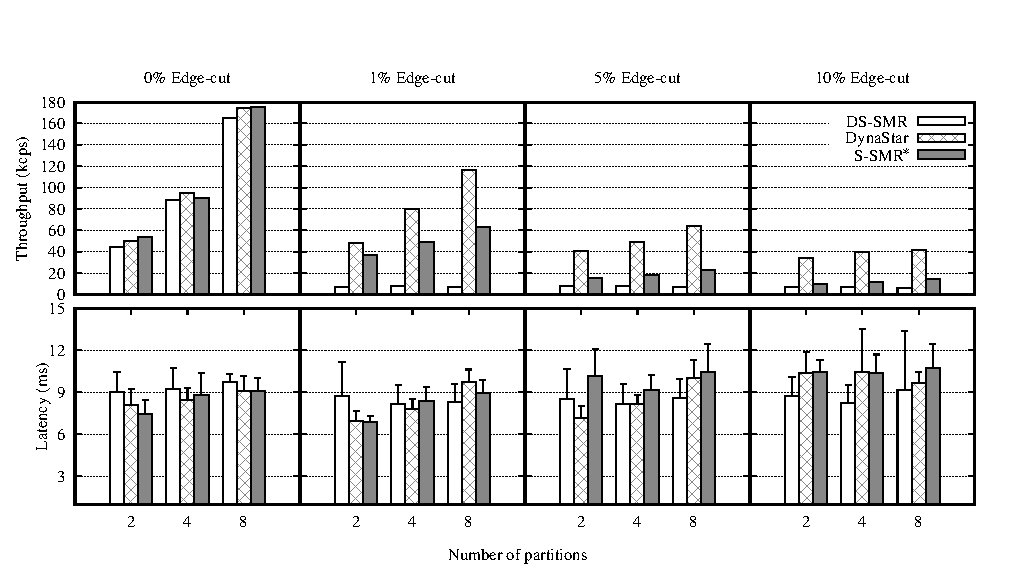
\includegraphics{figures/socc/socc-throughput-latency-avg-all}
	\caption{Throughput and latency, varying edge-cuts for different partitioning size. 
  Throughput is shown in thousands of commands per second (kcps). 
  Latency is measured in milliseconds (bars show average and whiskers show 95-th percentile).}
	\label{fig:varying_edge_cut}
\end{figure*}



\paragraph*{Performance metrics}
%
The latency was measured as the end-to-end time between issuing the
command, and receiving the response.  Throughput was measured as the
number of posts/second that the clients were able to send.

\paragraph*{Operational parameters}
%
With post commands, the frequency of single-partition
vs. multi-partition commands depends on the number of partitions, the
geometry of the social graph, and the technique used to partition the
data. We ran experiments with 2, 4, and 8 partitions.  To vary the
geometry, we generated graphs with varying percentages of edge-cuts as
computed by METIS on a static graph. Our experiments used graphs with
0\%, 1\%, 5\% and 10\% of edge cuts. We configured METIS to keep the size of 
the most unbalanced partition up to 30\% more than the average partition size.
As already mentioned, we compared three strategies: \ssmr{}, \dssmr, and \dynastar.


\subsection{\dynastar vs. alternative systems}
\label{sec:evaluation:results}

Figure~\ref{fig:varying_edge_cut} shows the peak throughput and average latency of the three strategies, 
as we vary the number of partitions for social networks with different percentages of edge cuts.

All three techniques perform similarly on experiments with
strong locality, because there are no cross-partition commands after
the graph is perfectly partitioned. No more moves occur in
\dynastar or \dssmr, and no synchronization among partitions is
necessary for \ssmr in this case. 
Consequently, all three schemes scale remarkably well, and
the difference in throughput between each technique is due to the implementation of each one.
Although \dynastar and DS-SMR have comparable performance, they differ in an important way. 
As shown in Figure~\ref{fig:motivation} (top left graph) for 4 partitions, \dynastar converges 
to maximum throughput after 20 seconds from the beginning of the execution, while it takes 
DS-SMR (decentralized dynamic scheme) about 80 seconds to converge.

With social networks that exhibit weak locality (edge cut percentage greater than zero) \dssmr\ performance decreases significantly.  
This happens because with weak locality, objects in \dssmr\ are constantly being moved back and forth between partitions 
without converging to a stable configuration.%(see also Figure~\ref{fig:motivation}, graph on the bottom right, for 4 partitions). 
In contrast, for \dynastar and \ssmr with an optimized partitioning, we see that the throughput scales with the number of partitions up to 10\% of edge cuts. 
With 10\% of edge cuts and above, the overhead from moves (in \dynastar) and cross-partition commands (in S-SMR) outweighs the gains from additional partitions.

\begin{figure}[ht]
	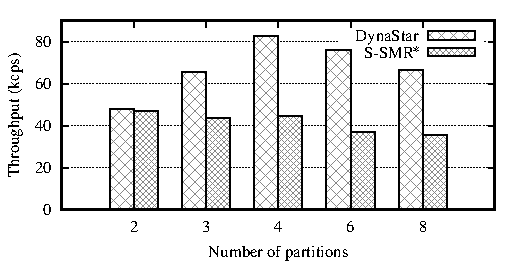
\includegraphics[width=0.95\columnwidth]{figures/socc/socc-throughput-avg-vary-partition}
	\caption{Performance of social graph with increasing partitions.}
	\label{fig:4p1p_varying_partition_size}
\end{figure}

\begin{figure*}[h!]
  \centering
  \begin{subfigure}[b]{0.45\textwidth}
    \centering
    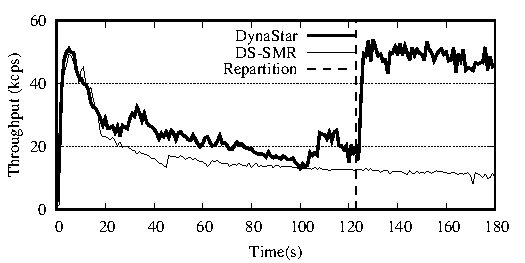
\includegraphics[width=0.95\columnwidth]{figures/socc/socc-dynamicload-tp}
    \caption{\dynastar versus DS-SMR}
  \end{subfigure}
  \begin{subfigure}[b]{0.45\textwidth}
    \centering
    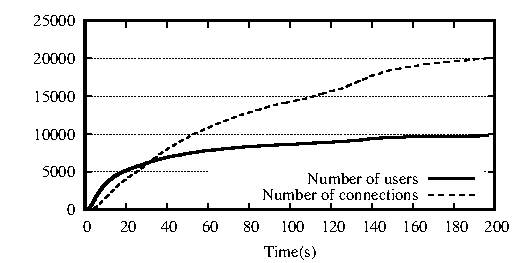
\includegraphics[width=0.95\columnwidth]{figures/socc/socc-dynamicload-graph}
    \caption{The creation of a social network graph}
  \end{subfigure}
    \caption{Performance under dynamic workload.}
	\label{fig:dynamic_load_tput}
\end{figure*}

% We can draw similar results about the latency of the three strategies (Figure~\ref{fig:varying_edge_cut}, graphs on the bottom).
% The large number of move operations in DS-SMR with social graphs that cannot be perfectly partitioned result in increased latency.


\subsection{The ideal number of partitions}
\label{sec:evaluation:results}

While in the previous section we considered executions with a fixed percentage of edge cuts.
%, as we increased the number of partitions 
%(by adjusting the social graph clustering coefficient),
We now consider a fixed graph and vary the number of partitions.
Increasing the number of partitions with a fixed graph introduces a tradeoff.
On one hand, additional partitions improve performance as there are more resources to execute posts.
On the other hand, the number of edge cuts increases with the number of partitions, which hurts performance as there are additional moves.
We evaluate the performance of \dynastar and \ssmr with an optimized partitioning.% when subject to this tradeoff. 

Figure~\ref{fig:4p1p_varying_partition_size} shows that throughput scales with the number of partitions until partitioned in more than 6 partitions.
For each configuration, we computed the percentage of edge cuts and found that for 2, 3, 4, 6 and 8 partitions the percentages were respectively 
0.13\%, 0.88, 1.06\%, 2.28\% and 2.67\%.
Notice that only post operations are subject to this tradeoff since they may involve multiple partitions.
The most common operation in social networks is the request to read a user timeline. This is a single-partition
command in our application and as a consequence it scales linearly with the number of partitions.


\subsection{Performance under dynamic workloads}

Figure~\ref{fig:dynamic_load_tput} (left) depicts dynamically repartitioning
on-the-fly.  We started the system with an empty graph. Then clients
continuously create users and connections between them during the experiment
by executing the follow command.
The rate at which users and connections are created is shown in Figure~\ref{fig:dynamic_load_tput} (right).
The oracle monitors changes in the
graph's structure and was configured to trigger a repartitioning after receiving a number of hints
%(object creating and connecting)
from the partitions.
%after all users were in the system and after 300 seconds into the execution.
%when the number of changes exceed a threshold.  
%When the repartitioning took place, the partitioning became better and helped the throughput increase.
%We also show the behavior of DS-SMR.
When the repartitioning took place, the previously random user mapping got a better location from the oracle.
After the repartitioning, the clients triggered the users to move to a better partition. 
The partitioning became better and thus the throughput increased.
We also show the behavior of DS-SMR.
When few connections are in the system, most of the posts are single-partition commands, but as connections are added, moves are needed to execute posts and performance decreases quickly.

%\begin{figure}[ht]
%	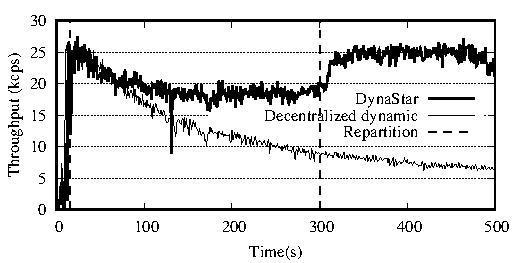
\includegraphics{figures/experiments/dynamicload-tp-move-4p}
%	\caption{Adding nodes and repartitioning dynamically}
%	\label{fig:dynamic_load_tput}
%\end{figure}
%\begin{figure}[ht]
%	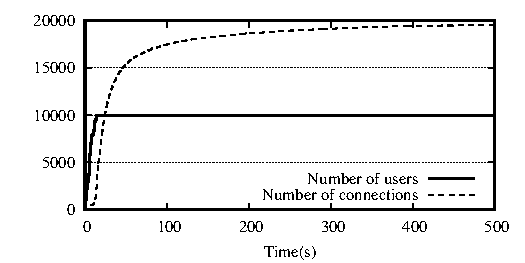
\includegraphics{figures/experiments/dynamicload-graph-structure}
%	\caption{Changes in dynamic workloads}
%	\label{fig:dynamic_load_changes}
%\end{figure}

\subsection{The performance of the oracle}

\dynastar differs from \dssmr\ in that it uses a centralized oracle
that maintains a global view of the workload graph. The oracle allows
\dynastar to make better choices about data movement, resulting in an overall
better throughput and lower latency. However, introducing a centralized
component in a distributed system is always a cause for some skepticism,
in case the component becomes a bottleneck, or a single point of failure. 
We therefore setup the oracle as a replicated partition 
and conducted two experiments to evaluate if the \dynastar oracle is a bottleneck to
system performance. The results show that the load on the oracle is
low, suggesting that \dynastar scales well.


The first experiment assesses the scalability of the METIS algorithm only.
We measured the time to compute the partitioning solution, and
the memory usage of the algorithms for increasingly large graphs. 
The results, depicted in Figure~\ref{fig:metis_size_time}, show that METIS scales
linearly in both memory and computation time on graphs of up to 10 million vertices.

\begin{figure}[ht!]
  \centering
    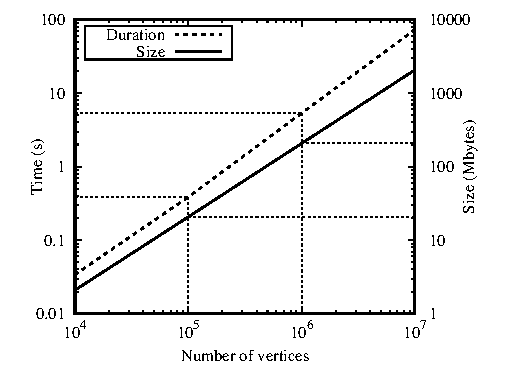
\includegraphics[width=\columnwidth]{figures/metis_size_time}
	\caption{METIS processor and memory usage.}
	\label{fig:metis_size_time}
\end{figure}

The second experiment evaluates the oracle in terms of CPU load over
time, for varying numbers of partitions. The results are shown in
Figure~\ref{fig:cpu_oracle}. The load is higher in the
beginning of the experiment, when the clients had not yet cached the
requests and the oracle was busy moving the state. However, the load diminishes rapidly, and remains relatively
low over time. This is because access to the oracle is necessary only
when clients have an invalid cache or when a repartition happens. This experiments
suggest that the oracle would not become a bottleneck.% for reasonably large
%deployments.

\begin{figure}[ht]
	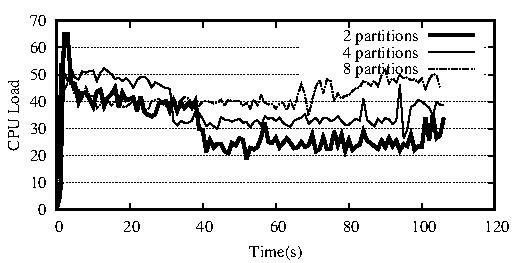
\includegraphics[width=\columnwidth]{figures/socc/socc-oracle-load}
	\caption{CPU load in the oracle.}
	\label{fig:cpu_oracle}
\end{figure}


%!TEX root =  main.tex
\section{Related work}
\label{sec:rw}

State machine replication~\cite{Kapritsos:2012um, kotla2004htbft, Lam78, santos2013htsmr, Sch90} provides strong consistency guarantees, which come from total order and deterministic execution of commands.
%Deterministic execution is usually ensured by having every replica execute commands sequentially.
Since consistent ordering is fundamental for SMR, some authors proposed to optimize the ordering and propagation of commands.
% (i.e., the atomic broadcast layer of the system).
For instance, \cite{kapritsos2010scalable} proposes to divide the ordering of commands between different clusters: each cluster orders only some requests, and then forwards the partial order to every server replica, which then merges the partial orders deterministically into a single total order that is consistent across the system.
In~\cite{biely2012spaxos}, Paxos~\cite{Lamport:1998ea} is used to order commands, but it is implemented in a way that avoids overloading the leader process, which would turn it into a bottleneck.

Multi-threaded execution is a potential source of non-determinism, depending on how threads are scheduled to be executed in the operating system.
Some works attempted to circumvent this problems and come up with a multi-threaded, yet deterministic implementation of SMR.
In \cite{santos2013htsmr}, the authors propose to parallelize the receipt and dispatching of commands, while executing commands sequentially.
In \cite{kotla2004htbft}, application semantics is used to determine which commands can be executed concurrently and still produce a deterministic outcome (e.g., read-only commands).
In \cite{Kapritsos:2012um}, commands are tentatively executed in parallel.
After the parallel execution, replicas verify whether they reached a consistent state; if not, commands are rolled back and re-executed sequentially.

Many database replication schemes aim at achieving high throughput by relaxing consistency, that is, they do not ensure linearizability.
In deferred-update replication \cite{chundi96dur, kobus2013hybrid, sciascia2012sdur, SousaOMP01}, replicas commit read-only transactions immediately, not always synchronizing with each other.
Although this indeed improves performance, it allows non-linearizable executions.
Database systems usually ensure serializability \cite{BHG87} or snapshot isolation \cite{LinKJPA09}, which do not take into account real-time precedence of different commands among different clients. 
For some applications, these consistency levels may be enough, allowing the system to scale better, but services that require linearizability cannot be implemented with such techniques.

Efforts to make linearizable systems scalable have been made in the past~\cite{bezerra2014ssmr, corbett2013spanner, Glendenning2011, hoang2016, Marandi:2011dj}.
In \cite{Glendenning2011}, the authors propose a scalable key-value store based on DHTs, ensuring linearizability, but only for requests that access the same key. 
In \cite{Marandi:2011dj}, variant of SMR is proposed in which data items are partitioned but commands have to be totally ordered.
Spanner~\cite{corbett2013spanner} uses a separate Paxos group per partition and, to ensure strong consistency across partitions, clocks are assumed to be synchronized.
Although the authors say that Spanner works well with GPS and atomic clocks, if clocks become out of synch beyond tolerated bounds, correctness is not guaranteed.
$M^2Paxos$~\cite{7579738} proposes a scheme where leases are used instead of partitions owning objects, but assumes full state replication.
\ssmr{}~\cite{bezerra2014ssmr} ensures consistency across partitions without any assumption about clock synchronization, but relies on a static partitioning of the state.
\dssmr{}~\cite{hoang2016} extends \ssmr\ by allowing state variables to migrate across partitions in order to reduce multi-partition commands.
However, \dssmr{} implements repartitioning in a very simple way that does not perform very well in scenarios where the state cannot be perfectly partitioned.
\dynastar\ improves on \dssmr\ by employing well-known graph partitioning techniques to decide where each variable should be.
Moreover, \dynastar\ dillutes the cost of repartitioning by moving variables on-demand, that is, only when they are accessed by some command.

Graph partitioning is an interesting problem with many proposed solutions~\cite{Abou-Rjeili:2006,hendrickson2000graph,kernighan1970efficient,7004087}.
In this work, we do not introduce a new graph partitioning solution, but instead we use a well-known one (METIS~\cite{Abou-Rjeili:2006}) to partition the state of a service implemented with state machine replication.
Similarly to \dynastar{}, Schism~\cite{curino2010sch} and Clay~\cite{SerafiniTEPAS16} also use graph-based partitioning to decide where to place data items in a transactional database.
In either case, not much detail is given about how to handle repartitioning dynamically without violating consistency.
Turcu et al. ~\cite{7004087} proposed a technique that reduces the amount of cross-partition commands and implements an advanced transaction routing.
Sword~\cite{quamar2013sword} is another graph-based dynamic repartitioning technique.
It uses a hypergraph partitioning algorithm to distribute rows of tables in a relational database across database shards.
Sword does not ensure linearizability and it is not clear how it implements repartitions without violating consistency.
E-Store~\cite{taft2014est} is yet another repartitioning proposal for transactional databases.
It repartitions data according to access patterns from the workload.
It strives to minimize the number of multi-partition accesses and is able to redistribute data items among partitions during execution.
E-Store assumes that all non-replicated tables form a tree-schema based on foreign key relationships.
This has the drawback of ruling out graph-structured schemas and \mbox{$m$-$n$} relationships.
\dynastar\ is a more general approach that works with any kind of relationship between data items, while also ensuring linearizability.

Some replication schemes are ``dynamic'' in that they allow the membership to be reconfigured during execution (e.g., \cite{birman2010dsr,dustdar2007soc,guessoum2003dar}).
For instance, a multicast layer based on Paxos can be reconfigured by adding or removing acceptors. 
These systems are dynamic in a way that is orthogonal to what \dynastar\ proposes.
%\dynastar\ consists of allowing the \emph{state partitioning}, that is, which state variables belong to which partition, to change dynamically.
%The greatest challenge that is addressed by \dynastar\ is how to provide such a solution, with a dynamic partitioning oracle, while ensuring a very strong level of consistency (linearizability), as variables are created, deleted, and moved across partitions, based on the access patterns of the workload.


\section{Conclusion}
\label{sec:conclusion}

This work introduces \dssmrlong{} (\dssmr), a scalable variant of the well-known
state machine replication technique. \dssmr{} implements dynamic state
partitioning to adapt to different access patterns throughout the execution,
while scaling throughput with the number of partitions and ensuring
linearizability. To evaluate \dssmr{}, we developed the \libname\ library and
implemented \appname{}, a scalable social network application, with \libname{}.
In our experiments, we deployed \appname\ with both \dssmr\ and \ssmr{}.
%, executing the application under workloads with weak and strong locality.
The results demonstrate that \dssmr\ significantly improves the performance of
\appname\ over \ssmr\ in the presence of multi-partition commands.
%, specially for workloads with strong locality.

%\clearpage

%%!TEX root =  main.tex
\subsection{Correctness}
\label{sec:correctness}

\newcommand{\tsc}{\ensuremath{t^{cli}_{start}}}
\newcommand{\tec}{\ensuremath{t^{cli}_{end}}}
\newcommand{\tes}{\ensuremath{t^{srv}_{end}}}
\newcommand{\tss}{\ensuremath{t^{srv}_{start}}}


In this section, we argue that \dynastar is safe (i.e., it ensures linearizability) and live (i.e., it ensures termination).

To prove that \dynastar ensures linearizability, we must show that for any execution $\sigma$ of the system, there is a total order $\pi$ on client commands that 
(i)~respects the semantics of the commands, as defined in their sequential specifications, and 
(ii)~respects the real-time precedence of commands~(Section~\ref{sec:correctcrit}).
%
Let $\pi$ be a total order of operations in $\sigma$ that respects $<$, the order atomic multicast induces on commands.

To argue that $\pi$ respects the semantics of  commands, let $C_i$ be the $i$-th command in $\pi$ and $p$ a process in partition $\ppm_p$ that executes $C_i$.
%Let $C_i$ be the $i$-th command in $\pi$ and $p$ a process in partition $\ppm_p$ that executes $C_i$.
We claim that when $p$ executes $C_i$, it has updated values of variables in $vars(C_i)$, the variables accessed by $C_i$.
We prove the claim by induction on $i$.
The base step trivially holds from the fact that variables are initialized correctly.
Let $v \in vars(C_i)$, $C_v$ be the last client command before $C_i$ in $\pi$ that accesses $v$, and $q$ a process in $\ppm_q$ that executes $C_v$.
From the inductive hypothesis, $q$ has an updated value of $v$ when it executes $C_v$.
There are two cases to consider:
(a)~$p = q$. In this case, $p$ obviously has an updated value of $v$ when it executes $C_i$ since no other command accesses $v$ between $C_v$ and $C_i$.
(b)~$p \neq q$. 
Since processes in the same partition execute the same commands, it must be that $\ppm_p \neq \ppm_q$.
From the algorithm, when $q$ executes $C_v$, $v \in \ppm_q$ and when $p$ executes $C_i$, $v \in \ppm_p$.
Thus, $q$ executed a command to move $v$ to another partition after executing $C_v$ and $p$ executed a command to move $v$ to $\ppm_p$ before executing $C_i$.
Since there is no command that accesses $v$ between $C_v$ and $C_i$ in $\pi$, $q$ has an updated $v$ when it executes $C_v$ (from inductive hypothesis), and $p$ receives the value of $v$ at $q$, it follows that $p$ has an updated $v$ when it executes $C_i$.

% DISCLAIMER: in the proof below, I assumed a single process per partition. While I'm pretty sure it works for multiple processes per partition, in some future refinement this should be added to the proof. Also see related picture showing cases (a) and (b) below. Perhaps we should include such a picture too in a future version.
%
We now argue that there is a total order $\pi$ that respects the real-time precedence of commands in $\sigma$.
Assume $C_i$ ends before $C_j$ starts, or more precisely, the time $C_i$ ends at a client is smaller than the time $C_j$ starts at a client, $\tec(C_i) < \tsc(C_j)$.
Since the time $C_i$ ends at the server from which the client receives the response for $C_i$ is smaller than the time $C_i$ ends at the client, $\tes(C_i) < \tec(C_i)$, and the time $C_j$ starts at the client is smaller than the time $C_j$ starts at the first server, $\tsc(C_j) < \tss(C_j)$, we conclude that $\tes(C_i) < \tss(C_j)$.

We must show that either $C_i < C_j$; or neither $C_i < C_j$ nor $C_j < C_i$.
For a contradiction, assume that $C_j <  C_i$ and let $C_j$ be executed by partition $\ppm_j$.

There are two cases: 
\begin{enumerate}
\item[(a)] $C_i$ is a client command executed by $\ppm_j$.
In this case, since $C_i$ only starts after $C_j$ at a server, it follows that $\tes(C_j) < \tss(C_i)$, a contradiction.
\item[(b)] $C_i$ is a client command executed by $\ppm_i$ that first involves a move of variables $vars$ from $\ppm_j$ to $\ppm_i$.
At $\ppm_j$, $\tes(C_j) < \tss(move(vars,\ppm_j,\ppm_i))$ since the move is only executed after $C_j$ ends.
Since the move only finishes when variables in $vars$ are in $\ppm_i$ and then $C_i$ can be executed, it must be that
$\tes(move(vars,\ppm_j,\ppm_i)) < \tss(C_i)$.
We conclude that $\tes(C_j) < \tss(C_i)$, a contradiction.
\end{enumerate}
Therefore, either $C_i < C_j$ and from the definition of $\pi$, $C_i$ precedes $C_j$ or neither $C_i < C_j$ nor $C_j < C_i$, and there is a total order in which $C_i$ precedes $C_j$.
%\begin{figure}
%\centering
%\includegraphics[width=1.2\linewidth,angle=-90]{figures/IMG_7203.JPG}
%\caption{Two cases in proof.}
%\end{figure}

For termination, we argue that every correct client eventually receives a reply different than $retry$ for every command $C$ that it issues.
This assumes that every partition (including the oracle partition) is always operational, despite the failure of some servers in the partition.
For a contradiction, assume that some client submits a command $C$ that always returns $retry$.
Therefore, from the algorithm, whenever $C$ is delivered at a partition, the partition does not contain all the variables needed by $C$.
As a consequence, the client eventually falls back to \ssmr\ and multicasts $C$ to all partitions and $C$ is executed as a multi-partition command, which is guaranteed to succeed, a contradiction that concludes our argument.





%\pagebreak

% why did you have this vvv ?
%\bibliographystyle{splncs03}


\bibliographystyle{abbrv}
\bibliography{references}

\end{document}
